This problem is designed to assess your ability to compute the forward kinematics (FK) of a serial
chain manipulator. Specifically, you will be computing the forward kinematics of the manipulator arm
of a KUKA youBot. Appendix \ref{app:kinematics} provides a design specification for the youBot arm.
Please note that the design specification gives lengths in millimeters, but the V-REP simulator uses
meters.

To complete this problem, design a ROS service named \texttt{fk} that computes the forward
kinematics for a given arm configuration. Take a look at \texttt{srv/Fk.srv} for the proper
input and output types of your service. You may find it helpful to first derive the
Denavit-Hartenberg parameters of the youBot arm. If you need a refresher on DH parameters or forward
kinematics, \href{https://rpal.cs.cornell.edu/foundations/kinematics.pdf#subsection.3.7}{these
notes} may be helpful.

Note that the return value of \texttt{fk} has type \texttt{PointArray}, which we define for you. Points in this array, which have type \texttt{geometry\_msgs/Point}, are interpreted as the positions of the origins of the arm link frames. Since there are five links in the youBot arm (not including the base), you should put the five origins in the array. For each of the five points in the array, a ball of a different size and color will be displayed in the simulator so that you can see where your \texttt{fk} service believes that each link is located. The final point in the array should be the position of the end-effector.

All of your code for this problem should go in the provided \texttt{src/fk.py} file.
Additionally, \texttt{fk.launch} is completed for you.

\vspace{16pt}
\begin{figure}[h]
  \centering
  \begin{subfigure}[b]{0.475\textwidth}
    \centering
    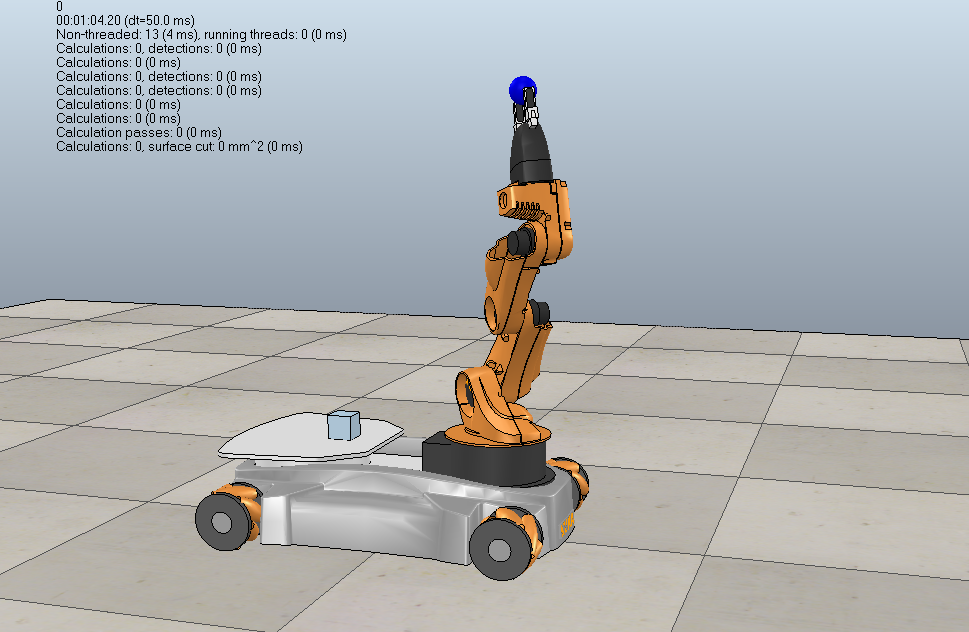
\includegraphics[width=\textwidth]{figures/p2/problem1.png}
    \caption[]%
    {{\small Correct FK calculation}}
    \label{fig:1a}
  \end{subfigure}
  \hfill
  \begin{subfigure}[b]{0.475\textwidth}
    \centering
    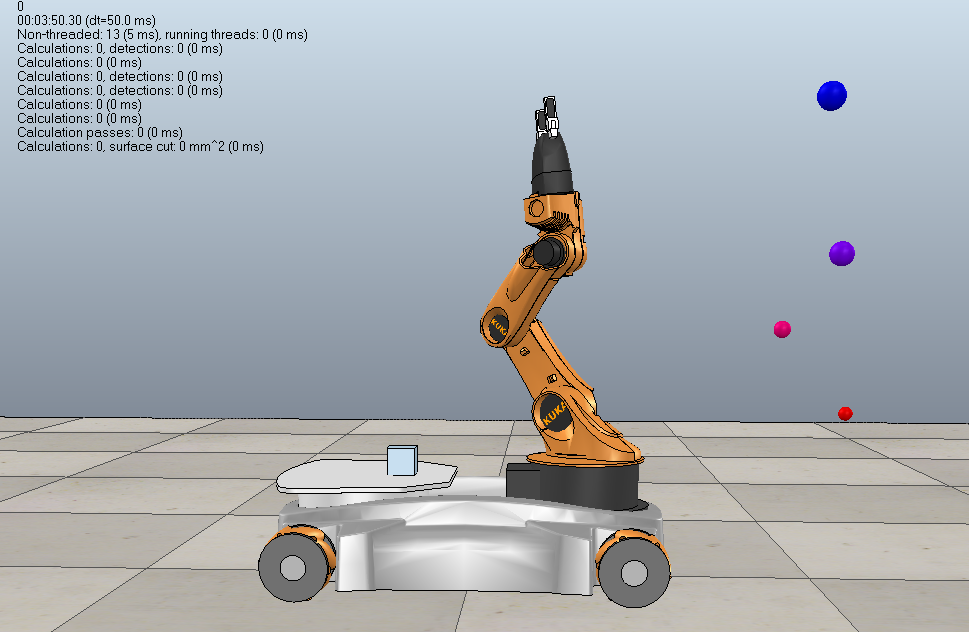
\includegraphics[width=\textwidth]{figures/p2/problem1_debug.png}
    \caption[]%
    {{\small Running in debug mode}}
    \label{fig:1b}
  \end{subfigure}
  \caption{Visualization of forward kinematics calculations. Image (\subref{fig:1a}) shows a correct
    FK calculation with debug mode turned off; note that the blue ball is between the fingers of the
  end-effector. Image (\subref{fig:1b}) shows an example of running the problem in debug mode.}
  \label{fig:1}
\end{figure}

When you run this problem, you will see that the arm moves quickly to a series of random
configurations. If your implementation of the \texttt{fk} service is correct, then you will see a
blue ball between the youBot fingers.

If your implementation has a bug, then it may be difficult to determine from the simulation what is
wrong because the arm moves rapidly. We have therefore provided you with a debug mode. In the file
\texttt{fk.launch}, there is a ROS parameter named \texttt{fk\_debug} that is set to
\texttt{False} by default. When it is set to \texttt{True}, the arm will move slowly through the
entire range of each joint. Furthermore, each ball showing your FK solution will be offset 0.4
meters in front of the robot. If you provide the positions of all five frame origins in the return
value of \texttt{fk}, then using debug mode will help you identify mistakes in your implementation.

